\documentclass{standalone}
\usepackage{tikz}
\usetikzlibrary{patterns}

\begin{document}

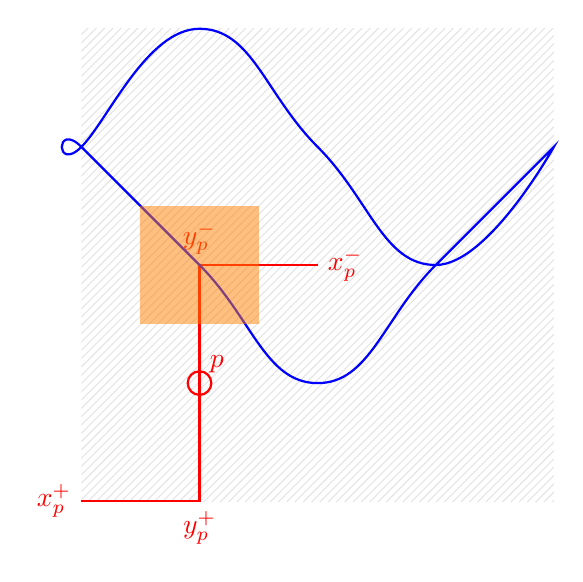
\begin{tikzpicture}[scale=1.5]
    % Define the pixel p
    \coordinate (p) at (0,0);
    
    % Draw the pixel grid
    \fill[pattern=north east lines, pattern color=gray!20] (-1,-1) rectangle (3,3);
    
    % Draw the pixel p with a cross
    \draw[red, thick] (p) circle (0.1) node[above right] {$p$};
    \draw[red, thick] (p) -- ++(0,1) node[above] {$y_p^-$} -- ++(1,0) node[right] {$x_p^-$};
    \draw[red, thick] (p) -- ++(0,-1) node[below] {$y_p^+$} -- ++(-1,0) node[left] {$x_p^+$};
    
    % Draw the boundary of the poorly textured region
    \draw[blue, thick] plot [smooth cycle,tension=0.8] coordinates {(-1,2) (0,3) (1,2) (2,1) (3,2) (2,1) (1,0) (0,1) (-1,2)};
    
    % Highlight the potential error pixels
    \fill[orange, opacity=0.5] (-0.5,0.5) rectangle (0.5,1.5);
    
\end{tikzpicture}

\end{document}